\documentclass[conference]{IEEEtran}
\IEEEoverridecommandlockouts

\usepackage{cite}
\usepackage{amsmath,amssymb}
\usepackage{graphicx}
\usepackage{algorithm}
\usepackage{algorithmic}
\usepackage[caption=false,font=footnotesize]{subfig}
\usepackage{xcolor}
\usepackage{tikz}
\usetikzlibrary{positioning,arrows.meta,decorations.pathreplacing,calc}

\newtheorem{definition}{Definition}
\newtheorem{proposition}{Proposition}
\newtheorem{remark}{Remark}

\DeclareMathOperator*{\argmax}{arg\,max}
\newcommand{\Qinv}{\mathsf{Q}^{-1}}
\newcommand{\Vsf}{\mathsf{V}}
\newcommand{\Csf}{\mathsf{C}}
\newcommand{\Hs}{\mathcal{H}}
\newcommand{\Ls}{\mathcal{L}}
\newcommand{\Ms}{\mathcal{M}}
\newcommand{\Rs}{\mathcal{R}}
\newcommand{\Bern}{\mathrm{Bern}}
\newcommand{\BSC}{\mathrm{BSC}}

% Red notes in the PDF. "Note:" marks information missing from the thesis; "Review:" marks
% suggested improvements. To hide them, replace either definition with \newcommand{...}[1]{}.
\newcommand{\authornote}[1]{{\color{red}\footnotesize[\textbf{Note:} #1]}}
\newcommand{\reviewnote}[1]{{\color{red}\footnotesize[\textbf{Review:} #1]}}

\begin{document}

\title{Finite-Blocklength Construction of Polar Superposition Codes for the Binary Symmetric Broadcast Channel}

\author{\IEEEauthorblockN{Paul Sheldon, Natasha Devroye, and Besma Smida}
\IEEEauthorblockA{Department of Electrical and Computer Engineering, University of Illinois Chicago, Chicago, IL, USA}}

\maketitle

\begin{abstract}
Superposition coding achieves the capacity region of the degraded binary symmetric broadcast channel (BSBC), and Goela, Abbe, and Gastpar showed that a polar-coded form of superposition coding does so with low complexity. Their construction is asymptotic: the message-carrying synthetic channels are defined through two polarization sets whose boundaries are only unambiguous as the blocklength grows. We study how to build polar superposition codes at practical blocklengths. First, we give a normal approximation for random superposition coding on the two-user BSBC under per-user reliability constraints, with closed-form dispersions and the correlation between the two successive-decoding stages at the strong receiver. Second, we show by example that selecting synthetic channels by relaxing the asymptotic polarization thresholds can be suboptimal, and we propose a low-complexity alternative that chooses the superposition parameter from the normal approximation and places message bits using the 5G NR reliability sequence. At blocklength $n=128$, the resulting codes outperform joint encoding of both messages at most of the evaluated rate pairs but fall short of time-division multiplexing (TDM). The normal approximation shows that this shortfall is inherent: even with random coding, superposition does not outperform TDM on the considered channel until $n=2^{11}$, and its advantage remains small up to $n=2^{20}$.
\end{abstract}
\reviewnote{The main finding is negative: on this channel, SUP cannot beat TDM at practical blocklengths, even with random coding. Consider a title that leads with it, e.g., ``When Does Superposition Pay Off? Polar Superposition Codes for the BSBC at Finite Blocklength.''}


\begin{IEEEkeywords}
Polar codes, superposition coding, broadcast channel, finite blocklength, normal approximation.
\end{IEEEkeywords}

\section{Introduction}
Renewed interest in non-orthogonal multiple access has brought superposition coding (SUP), one of its fundamental techniques, back into focus~\cite{7676258,9154358}. SUP achieves the capacity region of the degraded broadcast channel (BC)~\cite{CoverBC,ElGamalKim:book}, but the classical proof relies on random codebooks. For binary-input channels, Goela, Abbe, and Gastpar~\cite{6975233} showed that a superposition of two polar codes achieves the superposition region with encoding and decoding complexity $O(n\log n)$; Mondelli \emph{et al.}~\cite{mondelli2015marton} obtained a similar result for Marton's region. For Gaussian non-orthogonal multiple access (NOMA), Dai \emph{et al.}~\cite{dai2018pcnoma} designed polar-coded schemes that decompose the multiuser channel into polarized bit channels.

These constructions are asymptotic; the finite-length experiments in~\cite{6975233} concern a deterministic BC, not superposition coding. Polarization is also slow: the gap to capacity of polar codes shrinks only polynomially in the blocklength~\cite{hassani2014scaling}. Even for point-to-point (P2P) polar codes, choosing the information-carrying synthetic channels at finite blocklength is not fully solved, although there only a single reliability metric must be ranked: efficient estimation methods exist~\cite{talvardy2013}, and 5G NR standardizes a channel-independent reliability sequence~\cite{3gpp38212,bioglio2021}. A polar superposition code raises two additional design questions. The first is the choice of the superposition distribution, which determines how often the satellite codeword disturbs the cloud center. The second is that every satellite position must satisfy two criteria at once: it must have high entropy with respect to the code construction and low entropy with respect to the channel. As the blocklength grows, polarization makes the set satisfying both criteria unambiguous; at practical blocklengths, incomplete polarization makes the criteria conflict. Choi and Chung~\cite{CHOI2017111} design superposition polar codes for less-noisy BCs, but at blocklengths where the main difficulty is the estimation of Bhattacharyya parameters, as in the P2P case.

To judge what a practical code should achieve, we compare against finite-blocklength limits. Normal approximations~\cite{polyanskiy:TIT2010} have been derived for several network problems, including the asymmetric BC~\cite{Tan+Kosut} and the Gaussian multiple-access channel with degraded message sets~\cite{7289421ScarlettTanMACdegmsgset}. The dispersion of SUP has been studied for the Gaussian BC~\cite{unsal2017dispersion,wu2026dispersion,tuninetti2022second,9929397} and for unequal error protection~\cite{10622544}. In Gaussian downlink models, superposition-based NOMA often outperforms orthogonal multiple access at short blocklengths~\cite{sun2018shortpacket}, although not in every regime~\cite{amjad2020noma}. We find that the binary case behaves quite differently.

\emph{Contributions:} (i) We give a normal approximation for random SUP on the two-user BSBC with per-user reliability constraints, with closed-form dispersions and a closed-form correlation between the two successive-interference-cancellation (SIC) stages (Proposition~\ref{prop:na}). (ii) We interpret the satellite selection rule of~\cite{6975233} in terms of synthetic-channel reliability, and show at $n=16$ that relaxing the asymptotic thresholds can select a suboptimal position. (iii) We propose a construction that uses the normal approximation and the 5G NR reliability sequence, and evaluate it at $n=128$ against TDM and joint encoding. (iv) Using the normal approximation, we show that for the considered BSBC, SUP does not outperform TDM until $n=2^{11}$, which explains the behavior of the polar codes. \reviewnote{This claim is too strong. Read from Fig.~\ref{fig:n128}, the polar SUP points lie about $0.09$--$0.16$ bits/use below $\Rs^{\mathrm{SUP}}$ at the same $R_2$, while the realized TDM point lies about $0.07$ below $\Rs^{\mathrm{TDM}}$. Part of the shortfall is therefore a construction loss, not only SUP's inherent finite-blocklength penalty. Quantify both gaps in Sec.~\ref{sec:results}.}

\emph{Notation:} $[n]\triangleq\{1,\dots,n\}$; $x^{i:j}\triangleq(x_i,\dots,x_j)$ and $x^n\triangleq x^{1:n}$. Logarithms are base~2, $h(\cdot)$ is the binary entropy function, $a\star b\triangleq a(1-b)+(1-a)b$, $L(t)\triangleq\log\frac{1-t}{t}$, $\Csf(t)\triangleq 1-h(t)$ and $\Vsf(t)\triangleq t(1-t)L(t)^2$ are the capacity and dispersion of a $\BSC(t)$, and $\mathsf{Q}(\cdot)$ is the Gaussian complementary cumulative distribution function.

\section{System Model}
\begin{definition}[BSBC]
A $\mathrm{BSBC}(p_1,p_2)$ has input $X\in\{0,1\}$ and outputs $Y_j=X\oplus Z_j$, $j\in\{1,2\}$, where $Z_j\sim\Bern(p_j)$ is independent of $X$ and $0<p_1<p_2<\frac12$.
\end{definition}
Receiver~1 is the strong receiver, and the channel is stochastically degraded. Since we impose per-user reliability constraints, only the marginals $P_{Y_j|X}$ matter.
\reviewnote{Say why per-user rather than global (joint) reliability is used. Under a global constraint, the two receivers' information densities are correlated through the satellite (e.g., $\rho\approx0.6$ between $\imath_2$ and $\imath_{\mathrm c}$ for $\mathrm{BSBC}(0.01,0.10)$ with $\alpha=0.1$), so the two formulations give different regions.}


\begin{definition}[Code]
An $(n,M_1,M_2,\varepsilon_1,\varepsilon_2)$ code consists of an encoder $f:[M_1]\times[M_2]\to\{0,1\}^n$ and decoders $\phi_j:\{0,1\}^n\to[M_j]$ such that, for independent and uniformly distributed messages $(m_1,m_2)$, $\Pr[\phi_j(Y_j^n)\neq m_j]\leq\varepsilon_j$ for $j\in\{1,2\}$. A rate pair $(R_1,R_2)$ is $(n,\varepsilon_1,\varepsilon_2)$-achievable if such a code exists with $\log M_j\geq nR_j$.
\end{definition}

The capacity region of the BSBC is~\cite{ElGamalKim:book}
\begin{equation}
\Csf_{\mathrm{BC}}=\bigcup_{\alpha\in[0,\frac12]}\left\{(R_1,R_2):\begin{array}{l}R_1\leq h(\alpha\star p_1)-h(p_1)\\ R_2\leq 1-h(\alpha\star p_2)\end{array}\right\}.
\label{eq:capacity}
\end{equation}
It is achieved by SUP: cloud-center codewords $v^n(m_2)$ are drawn i.i.d.\ $\Bern(\frac12)$, and satellite codewords are $x^n(m_1,m_2)=v^n(m_2)\oplus s^n(m_1,m_2)$ with $s^n$ drawn i.i.d.\ $\Bern(\alpha)$. Equivalently, $X=V\oplus S$ with $S\sim\Bern(\alpha)$ independent of $V$, i.e., $P_{X|V}=\BSC(\alpha)$. The parameter $\alpha$ is the fraction of cloud-center bits flipped by the satellite. Receiver~2 decodes $m_2$ treating the satellite as noise, so that it observes $V$ through a $\BSC(q_2)$ with $q_j\triangleq\alpha\star p_j$. Receiver~1 uses SIC: it decodes $m_2$ through a $\BSC(q_1)$, and then $m_1$.

\section{Normal Approximation for Superposition Coding}
\label{sec:na}
The decoders operate on the information densities
\begin{align}
\imath_2(v;y)&=\log\frac{P_{Y_2|V}(y|v)}{P_{Y_2}(y)},\quad
\imath_{\mathrm c}(v;y)=\log\frac{P_{Y_1|V}(y|v)}{P_{Y_1}(y)},\nonumber\\
\imath_{\mathrm s}(x;y|v)&=\log\frac{P_{Y_1|X}(y|x)}{P_{Y_1|V}(y|v)},
\end{align}
for the weak receiver, the cloud stage of the strong receiver, and its satellite stage, respectively. Under the i.i.d.\ SUP distribution, $\imath_2$ has mean $\Csf(q_2)$ and variance $\Vsf(q_2)$. For the strong receiver, let $E=\mathbf{1}\{Y_1\neq V\}\sim\Bern(q_1)$ and $Z_1=\mathbf{1}\{Y_1\neq X\}\sim\Bern(p_1)$. Then
\begin{align}
\imath_{\mathrm c}&=1+\log(1-q_1)-E\,L(q_1),\nonumber\\
\imath_{\mathrm s}&=\log\tfrac{1-p_1}{1-q_1}-Z_1L(p_1)+E\,L(q_1).
\end{align}
Since $E=Z_1=1$ requires $S=0$, $\mathrm{Cov}(E,Z_1)=(1-\alpha)p_1-q_1p_1=(1-2\alpha)p_1(1-p_1)$, which gives
\begin{align}
I_{\mathrm c}&\triangleq\mathbb{E}[\imath_{\mathrm c}]=1-h(q_1),\quad
V_{\mathrm c}\triangleq\mathrm{Var}[\imath_{\mathrm c}]=\Vsf(q_1),\nonumber\\
I_{\mathrm s}&\triangleq\mathbb{E}[\imath_{\mathrm s}]=h(q_1)-h(p_1),\nonumber\\
V_{\mathrm s}&\triangleq\mathrm{Var}[\imath_{\mathrm s}]=\Vsf(p_1)+\Vsf(q_1)-2\kappa,\nonumber\\
V_{\mathrm{cs}}&\triangleq\mathrm{Cov}[\imath_{\mathrm c},\imath_{\mathrm s}]=\kappa-\Vsf(q_1),
\label{eq:moments}
\end{align}
where $\kappa\triangleq(1-2\alpha)p_1(1-p_1)L(p_1)L(q_1)$, and the correlation coefficient $\rho\triangleq V_{\mathrm{cs}}/\sqrt{V_{\mathrm c}V_{\mathrm s}}$.

\begin{proposition}[Normal approximation]
\label{prop:na}
Fix $\alpha\in(0,\frac12)$. Up to $O(\frac{\log n}{n})$ terms, random SUP with the decoders above achieves every $(R_1,R_2)$ that satisfies
\begin{subequations}
\label{eq:na}
\begin{align}
R_2&\leq\Csf(q_2)-\sqrt{\Vsf(q_2)/n}\;\Qinv(\varepsilon_2),\label{eq:na-weak}\\
R_2&\leq I_{\mathrm c}-\sqrt{V_{\mathrm c}/n}\;\Qinv(\varepsilon_{\mathrm c}),\label{eq:na-cloud}\\
R_1&\leq I_{\mathrm s}-\sqrt{V_{\mathrm s}/n}\;\Qinv(\varepsilon_{\mathrm s}),\label{eq:na-sat}
\end{align}
\end{subequations}
for some $(\varepsilon_{\mathrm c},\varepsilon_{\mathrm s})\in(0,1)^2$ with $\mathsf{F}(\varepsilon_{\mathrm c},\varepsilon_{\mathrm s};\rho)\geq1-\varepsilon_1$, where
\begin{multline*}
\mathsf{F}(a,b;\rho)\triangleq\Pr\big[G_1\leq\Qinv(a),\\ \rho G_1+\sqrt{1-\rho^2}\,G_2\leq\Qinv(b)\big]
\end{multline*}
and $G_1,G_2$ are i.i.d.\ standard Gaussian. We denote the union of these regions over $\alpha$ by $\Rs^{\mathrm{SUP}}(n,\varepsilon_1,\varepsilon_2)$.
\end{proposition}
\begin{IEEEproof}[Proof sketch]
Receiver~2 applies a threshold test to $\sum_k\imath_2(v_k(m);y_{2,k})$; the dependence-testing bound and the Berry--Esseen theorem give \eqref{eq:na-weak}, as for a P2P $\BSC(q_2)$~\cite{polyanskiy:TIT2010}. Receiver~1 applies a threshold test to $\sum_k\imath_{\mathrm c}$ over the cloud codewords, and then to $\sum_k\imath_{\mathrm s}$ over the satellite codewords of the decoded cloud center. An incorrect codeword passes either test with a probability that only affects the rates through $O(\frac{\log n}{n})$ terms. The true codewords pass both tests unless one of the two sums of i.i.d.\ vectors $(\imath_{\mathrm c},\imath_{\mathrm s})$, whose covariance is given by \eqref{eq:moments}, falls below its threshold. The multivariate Berry--Esseen theorem, as in~\cite{Tan+Kosut}, then gives the probability of correct decoding $\mathsf{F}(\varepsilon_{\mathrm c},\varepsilon_{\mathrm s};\rho)$ with the thresholds of \eqref{eq:na-cloud}--\eqref{eq:na-sat}.
\end{IEEEproof}
\reviewnote{Proposition~\ref{prop:na} specializes the asymmetric-BC analysis of~\cite{Tan+Kosut} and is only sketched, so reviewers may see it as incremental. Either give a complete proof (appendix or arXiv version), or present it as a normal approximation rather than a proposition and position the closed-form moments \eqref{eq:moments} as the contribution.}


\begin{remark}
Numerically, $\rho<0$ for all $(p_1,\alpha)\in(0,\frac12)^2$ (e.g., $\rho\approx-0.77$ for $p_1=0.01$, $\alpha=0.1$): an observation that disagrees with the cloud center ($E=1$) lowers $\imath_{\mathrm c}$ but raises $\imath_{\mathrm s}$, because the satellite's information is precisely the cloud stage's interference.
\end{remark}

As baselines, we use the normal approximations of TDM, in which user~1 receives a fraction $\lambda$ of the channel uses,
\begin{equation}
\Rs^{\mathrm{TDM}}=\bigcup_{\lambda\in[0,1]}\left\{(R_1,R_2):\begin{array}{l}R_1\leq r(\lambda,p_1,\varepsilon_1)\\R_2\leq r(1-\lambda,p_2,\varepsilon_2)\end{array}\right\},
\label{eq:tdm}
\end{equation}
where $r(\lambda,p,\varepsilon)\triangleq\lambda\Csf(p)-\sqrt{\lambda\Vsf(p)/n}\,\Qinv(\varepsilon)$, and of a common codeword (CCP) that carries both messages and is decoded by both receivers, $R_1+R_2\leq\min_j r(1,p_j,\varepsilon_j)$.

\section{Polar Superposition Codes}
\subsection{The Goela--Abbe--Gastpar Construction}
\label{sec:gag}
\begin{figure}[t]
\centering
\resizebox{\columnwidth}{!}{%
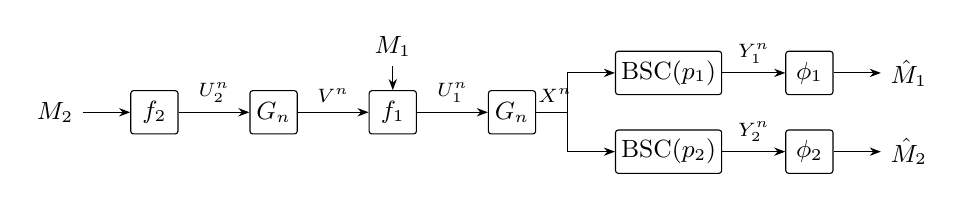
\begin{tikzpicture}[>={Stealth[length=4pt]}, node distance=4mm and 6mm,
  blk/.style={draw, rounded corners=1pt, minimum height=5.5mm, minimum width=6mm, inner sep=2pt, font=\small},
  lbl/.style={font=\small}, every edge quotes/.style={font=\scriptsize}]
  \node[lbl] (m2) {$M_2$};
  \node[blk, right=of m2] (f2) {$f_2$};
  \node[blk, right=9mm of f2] (g2) {$G_n$};
  \node[blk, right=9mm of g2] (f1) {$f_1$};
  \node[lbl, above=3mm of f1] (m1) {$M_1$};
  \node[blk, right=9mm of f1] (g1) {$G_n$};
  \node[blk, right=10mm of g1, yshift=5mm] (w1) {$\BSC(p_1)$};
  \node[blk, right=10mm of g1, yshift=-5mm] (w2) {$\BSC(p_2)$};
  \node[blk, right=8mm of w1] (d1) {$\phi_1$};
  \node[blk, right=8mm of w2] (d2) {$\phi_2$};
  \node[lbl, right=of d1] (o1) {$\hat M_1$};
  \node[lbl, right=of d2] (o2) {$\hat M_2$};
  \draw[->] (m2) -- (f2);
  \draw[->] (f2) -- node[above, font=\scriptsize] {$U_2^n$} (g2);
  \draw[->] (g2) -- node[above, font=\scriptsize] {$V^n$} (f1);
  \draw[->] (m1) -- (f1);
  \draw[->] (f1) -- node[above, font=\scriptsize] {$U_1^n$} (g1);
  \coordinate[right=4mm of g1] (split);
  \draw (g1) -- node[above, font=\scriptsize, pos=0.6] {$X^n$} (split);
  \draw[->] (split) |- (w1);
  \draw[->] (split) |- (w2);
  \draw[->] (w1) -- node[above, font=\scriptsize] {$Y_1^n$} (d1);
  \draw[->] (w2) -- node[above, font=\scriptsize] {$Y_2^n$} (d2);
  \draw[->] (d1) -- (o1);
  \draw[->] (d2) -- (o2);
\end{tikzpicture}}
\caption{Polar superposition coding for the BSBC~\cite{6975233}. The cloud center $V^n$ carries $M_2$; the satellite encoder $f_1$ uses $V^n$ to produce $X^n$, which carries $M_1$.}
\label{fig:blockdiagram}
\end{figure}

\reviewnote{This subsection restates~\cite{6975233} at length. Condensing it to the set definitions and the encoding rule would free space for the comparisons suggested in Sec.~\ref{sec:results}.} Fig.~\ref{fig:blockdiagram} shows the construction of~\cite{6975233}. Let $n=2^m$ and $G_n=\left[\begin{smallmatrix}1&0\\1&1\end{smallmatrix}\right]^{\otimes m}$ over $\mathbb{F}_2$, which satisfies $G_n^{-1}=G_n$. We omit the bit-reversal permutation of~\cite{ArikanPolar} and index positions as in 5G NR~\cite{3gpp38212}. For $(V^n,X^n,Y_1^n,Y_2^n)$ i.i.d.\ according to $P_VP_{X|V}P_{Y_1Y_2|X}$, define the cloud vector $U_2^n=V^nG_n$ and the satellite vector $U_1^n=X^nG_n$. With the Bhattacharyya parameter $Z(T|W)\triangleq2\sum_wP_W(w)\sqrt{P_{T|W}(0|w)P_{T|W}(1|w)}$ and $\delta_n=2^{-n^\beta}$, $\beta\in(0,\frac12)$, define
\begin{align}
\Hs_{V}&=\{i:Z(U_2(i)|U_2^{1:i-1})\geq1-\delta_n\},\nonumber\\
\Ls_{V|Y_2}&=\{i:Z(U_2(i)|U_2^{1:i-1},Y_2^n)\leq\delta_n\},\nonumber\\
\Hs_{X|V}&=\{i:Z(U_1(i)|U_1^{1:i-1},V^n)\geq1-\delta_n\},\nonumber\\
\Ls_{X|VY_1}&=\{i:Z(U_1(i)|U_1^{1:i-1},V^n,Y_1^n)\leq\delta_n\},
\label{eq:sets}
\end{align}
and the message sets $\Ms_2=\Hs_V\cap\Ls_{V|Y_2}$ and $\Ms_1=\Hs_{X|V}\cap\Ls_{X|VY_1}$. Because the BSBC is degraded, the positions in $\Ls_{V|Y_2}$ are also reliable at receiver~1~\cite{6975233}.

\emph{Encoding:} For $i=1,\dots,n$, $u_2(i)$ is the next bit of $m_2$ if $i\in\Ms_2$ and $\psi_2^{(i)}(u_2^{1:i-1})$ otherwise. Then $v^n=u_2^nG_n$. Next, $u_1(i)$ is the next bit of $m_1$ if $i\in\Ms_1$ and $\psi_1^{(i)}(u_1^{1:i-1},v^n)$ otherwise, and $x^n=u_1^nG_n$. We use the deterministic maps
\begin{align}
\psi_2^{(i)}(u_2^{1:i-1})&=\argmax_{u\in\{0,1\}}P_{U_2(i)|U_2^{1:i-1}}(u|u_2^{1:i-1}),\nonumber\\
\psi_1^{(i)}(u_1^{1:i-1},v^n)&=\argmax_{u\in\{0,1\}}P_{U_1(i)|U_1^{1:i-1}V^n}(u|u_1^{1:i-1},v^n),
\label{eq:psi}
\end{align}
with ties broken in favor of~0. The capacity proof of~\cite{6975233} uses randomized maps instead, but the experiments there found that a deterministic rule gives lower error probability in practice. Running an SC computation at the encoder in this way parallels the Honda--Yamamoto scheme for asymmetric channels~\cite{honda2013}. With $P_V=\Bern(\frac12)$, $U_2^n$ is i.i.d.\ uniform, so $\Hs_V=[n]$ and $\psi_2^{(i)}\equiv0$: the cloud center is an ordinary polar code for the $\BSC(q_2)$. The satellite's frozen positions, in contrast, are not fixed. Their values depend on $v^n$ and on the preceding bits of $u_1^n$, which steers $x^n$ to agree with $v^n$ except in a fraction of approximately $\alpha$ positions. Since $X^n$ is uniform and $V^n$ is $X^n$ observed through a $\BSC(\alpha)$, the probabilities in $\psi_1^{(i)}$ are exactly the successive-cancellation (SC) likelihoods of~\cite{ArikanPolar} for a $\BSC(\alpha)$ observation. They are therefore computed with the usual $O(n\log n)$ recursion from the channel log-likelihood ratios (LLRs) $(1-2v_k)\log\frac{1-\alpha}{\alpha}$.

\emph{Decoding:} Receiver $j$ SC-decodes $u_2^n$ from $y_j^n$ with LLRs $(1-2y_{j,k})\log\frac{1-q_j}{q_j}$ and frozen bits~0. Receiver~1 then forms $\hat v^n=\hat u_2^nG_n$ and SC-decodes $u_1^n$ with LLRs $(1-2\hat v_k)\log\frac{1-\alpha}{\alpha}+(1-2y_{1,k})\log\frac{1-p_1}{p_1}$, which combine the two observations because $V-X-Y_1$ is a Markov chain. For $i\notin\Ms_1$ it sets $\hat u_1(i)=\psi_1^{(i)}(\hat u_1^{1:i-1},\hat v^n)$, repeating the encoder's choice. \reviewnote{State the complexity cost. The encoder needs an SC likelihood recursion rather than XORs only, and the strong receiver runs about three SC recursions: one for $u_2^n$, and two for $u_1^n$ (with $V$-only and with $V$+$Y_1$ likelihoods). This is relevant when comparing with TDM.}

With $P_V=\Bern(\frac12)$, \cite{6975233} shows that $|\Ms_2|/n\to1-h(\alpha\star p_2)$ and $|\Ms_1|/n\to h(\alpha\star p_1)-h(p_1)$, which recovers \eqref{eq:capacity}, with error probability $O(2^{-n^\beta})$.

\subsection{Satellite Positions at Finite Blocklength}
\label{sec:selection}
The satellite sets have a simple interpretation. Given $V^n$, $U_1^n=V^nG_n\oplus S^nG_n$, so $H(U_1(i)|U_1^{1:i-1},V^n)$ is the conditional entropy of the polar-transformed Bernoulli($\alpha$) sequence $S^n$. Because $S^n$ is exactly the noise of a $\BSC(\alpha)$ with uniform input, this entropy equals $1-I(W_\alpha^{(i)})$ (cf.\ source polarization~\cite{arikan2010source}), where $W_\alpha^{(i)}$ is the $i$th synthetic channel of a $\BSC(\alpha)$. Hence $\Hs_{X|V}$ consists of the positions that are \emph{unreliable} for a $\BSC(\alpha)$. In contrast, $\Ls_{X|VY_1}$ consists of the positions that are \emph{reliable} for the channel from $X$ to $(V,Y_1)$, which is a $\BSC(\alpha)$ and a $\BSC(p_1)$ in parallel. A satellite position must therefore be unresolvable from the cloud center alone yet resolvable once receiver~1's observation is added. As $n\to\infty$, polarization makes both sets sharply defined. At short blocklengths, the positions that could serve the satellite are only partially polarized under both criteria.

\begin{figure*}[t]
\centering
\subfloat[$1-Z(U_1(i)|U_1^{1:i-1},V^n)$\label{fig:bhat-h}]{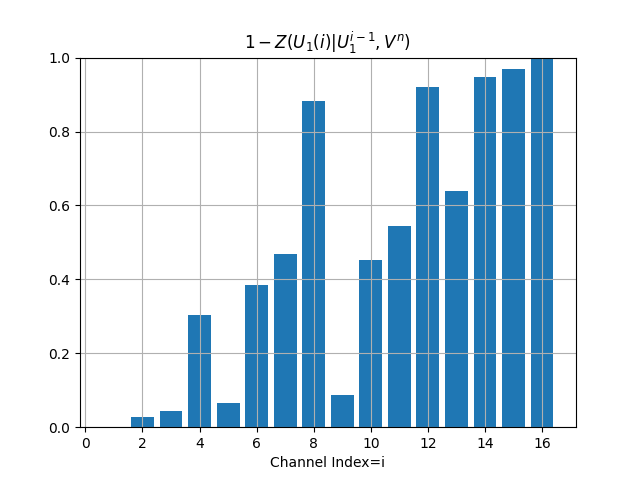
\includegraphics[width=0.42\textwidth,trim=20 4 40 8,clip]{figures/bhattacharyya_given_v.png}}\hspace{8mm}
\subfloat[$Z(U_1(i)|U_1^{1:i-1},V^n,Y_1^n)$\label{fig:bhat-l}]{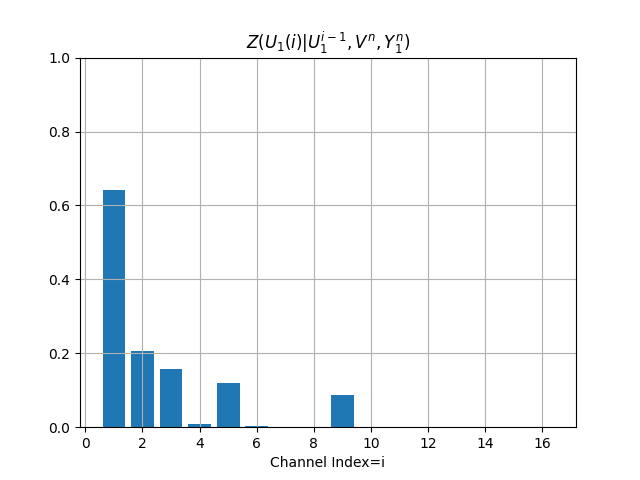
\includegraphics[width=0.42\textwidth,trim=20 4 40 8,clip]{figures/bhattacharyya_given_v_y1.png}}
\caption{Monte-Carlo estimates of the two selection metrics for the satellite positions, $n=16$, $\mathrm{BSBC}(0.01,0.10)$, $\alpha=0.10$. A good satellite position needs both values to be small.}
\label{fig:bhattacharyya}
\end{figure*}

Fig.~\ref{fig:bhattacharyya} illustrates this for $n=16$, $\mathrm{BSBC}(0.01,0.10)$, and $\alpha=0.1$. The positions with small $1-Z(U_1(i)|U_1^{1:i-1},V^n)$, namely $\{1,2,3,5,9\}$, are exactly the five least reliable positions of the 5G NR sequence. They are also the positions at which $Z(U_1(i)|U_1^{1:i-1},V^n,Y_1^n)$ is largest. No position makes both metrics close to zero.

A direct finite-blocklength version of the construction, which we call the baseline (Algorithm~\ref{alg:baseline}), keeps the single threshold of \eqref{eq:sets} and relaxes it until both message sets are large enough. For one information bit per user, $\Ms_2=\{16\}$, and $\delta$ must be relaxed to almost $0.1$ before any satellite position qualifies, which gives $\Ms_1=\{9\}$. The resulting code has a simulated total error probability of approximately $0.011$. However, the code with $\Ms_2=\{16\}$ and $\Ms_1=\{4\}$ achieves approximately $0.007$, even though position~4 is far from the high-entropy threshold ($1-Z\approx0.30$). Relaxing the asymptotic thresholds therefore does not identify the best positions. \authornote{Define ``total error probability'' and state the number of simulated blocks.} \reviewnote{Separating $0.011$ from $0.007$ at $3\sigma$ needs on the order of $10^4$ blocks per code; add confidence intervals. Also report what Algorithm~\ref{alg:na} selects here. With capacity-based sizing it gives $\bar k_1=\lfloor16\,\Csf(0.01)\rfloor=14$ and hence $\Ms_1=\{3\}$, where Fig.~\ref{fig:bhattacharyya}(b) shows $Z\approx0.16$, worse than the baseline's position~9.}

\begin{algorithm}[t]
\caption{Baseline selection}
\label{alg:baseline}
\begin{algorithmic}[1]
\REQUIRE $n$, $\alpha$, target sizes $k_1,k_2$; $P_V=\Bern(\frac12)$
\STATE Estimate the Bhattacharyya parameters in \eqref{eq:sets} by Monte-Carlo simulation~\cite[Sec.~IV-E]{6975233}
\STATE $\delta\gets0$
\WHILE{$|\Ms_1|<k_1$ \OR $|\Ms_2|<k_2$}
\STATE Increase $\delta$ and recompute \eqref{eq:sets} with $\delta$ in place of $\delta_n$
\ENDWHILE
\end{algorithmic}
\end{algorithm}

\subsection{Normal-Approximation-Assisted Construction}
\label{sec:proposed}
Algorithm~\ref{alg:na} avoids estimating Bhattacharyya parameters altogether. It uses Proposition~\ref{prop:na} to choose $\alpha$, sizes the message sets from the P2P rates of the two virtual channels, and places message bits according to the 5G NR reliability sequence $\pi_n$~\cite{3gpp38212,bioglio2021}, ordered from least to most reliable. The cloud positions are the most reliable positions, as in a P2P polar code for the $\BSC(q_2)$. The set $\mathcal{S}_1$ contains the positions that are reliable for receiver~1's P2P channel; these remain reliable when $V^n$ is also observed, so $\mathcal{S}_1$ approximates a subset of $\Ls_{X|VY_1}$. The least reliable positions of $\mathcal{S}_1$ are those closest to the unreliable set $\Hs_{X|V}$, so, under a common reliability order, the algorithm takes the satellite positions from the boundary between the two sets of Section~\ref{sec:selection}. Fig.~\ref{fig:selection} illustrates the result for $n=8$. \reviewnote{Steps~3--4 size the sets with capacities even though $\alpha$ comes from the finite-$n$ normal approximation; using the normal-approximation rates would be consistent. In addition, under a common reliability order the identity above implies that $\Hs_{X|V}\cap\Ls_{X|VY_1}$ is the band of $k_1$ positions \emph{ending} at rank $\approx n\,h(\alpha)$, whereas Algorithm~\ref{alg:na} \emph{starts} at rank $\approx n\,h(p_1)$. In the $n=16$ example, the better position~4 has rank~6, close to $n\,h(0.1)\approx7.5$. Compare the two anchors.}

\begin{algorithm}[t]
\caption{Normal-approximation-assisted selection}
\label{alg:na}
\begin{algorithmic}[1]
\REQUIRE $n$, $p_1$, $p_2$, $\varepsilon_1$, $\varepsilon_2$, target $k_1=nR_1$; reliability order $\pi_n$
\STATE $P_V\gets\Bern(\frac12)$
\STATE $\alpha\gets$ the value at which the boundary of $\Rs^{\mathrm{SUP}}(n,\varepsilon_1,\varepsilon_2)$ attains $R_1=k_1/n$ (Prop.~\ref{prop:na})
\STATE $k_2\gets\lfloor n\,\Csf(\alpha\star p_2)\rfloor$
\STATE $\bar k_1\gets\lfloor n\,\Csf(p_1)\rfloor$
\STATE $\Ms_2\gets$ the $k_2$ most reliable positions of $\pi_n$
\STATE $\mathcal{S}_1\gets$ the $\bar k_1$ most reliable positions of $\pi_n$
\STATE $\Ms_1\gets$ the $k_1$ least reliable positions of $\mathcal{S}_1$
\RETURN $\alpha$, $\Ms_1$, $\Ms_2$
\end{algorithmic}
\end{algorithm}

\begin{figure}[t]
\centering
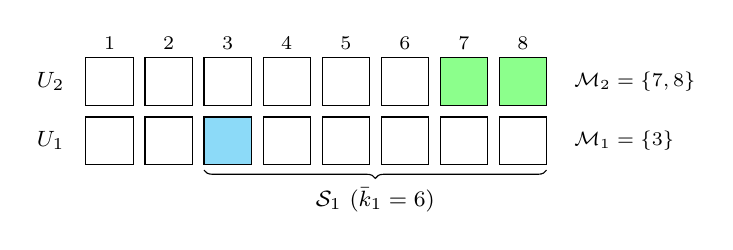
\begin{tikzpicture}[x=7.5mm, y=7.5mm, font=\footnotesize,
  cell/.style={draw, minimum size=6mm, inner sep=0pt},
  sel1/.style={cell, fill=cyan!45}, sel2/.style={cell, fill=green!45}]
  \node[anchor=east] at (0.4,1) {$U_2$};
  \node[anchor=east] at (0.4,0) {$U_1$};
  \foreach \i in {1,...,8} {
    \node[font=\scriptsize] at (\i,1.65) {\i};
    \ifnum\i>6 \node[sel2] at (\i,1) {}; \else \node[cell] at (\i,1) {}; \fi
    \ifnum\i=3 \node[sel1] at (\i,0) {}; \else \node[cell] at (\i,0) {}; \fi
  }
  \draw[decorate, decoration={brace, mirror, amplitude=3pt}] (2.6,-0.5) -- node[below=3pt] {$\mathcal{S}_1$ ($\bar k_1=6$)} (8.4,-0.5);
  \node[anchor=west, font=\scriptsize] at (8.7,1) {$\Ms_2=\{7,8\}$};
  \node[anchor=west, font=\scriptsize] at (8.7,0) {$\Ms_1=\{3\}$};
\end{tikzpicture}
\caption{Algorithm~\ref{alg:na} for $n=8$, $k_2=2$, $\bar k_1=6$, and $k_1=1$. The 5G NR order from least to most reliable is $(1,2,3,5,4,6,7,8)$, so $\Ms_2$ is its last two entries and $\Ms_1$ is the least reliable entry of $\mathcal{S}_1=\{3,\dots,8\}$.}
\label{fig:selection}
\end{figure}

\section{Numerical Results}
\label{sec:results}
\begin{figure}[t]
\centering
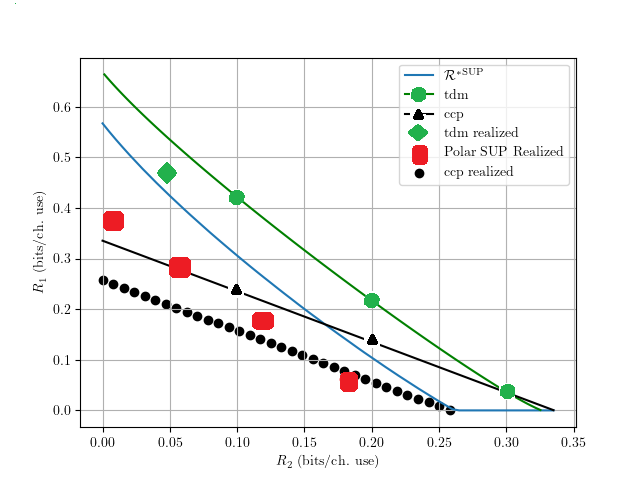
\includegraphics[width=\columnwidth,trim=10 0 40 25,clip]{figures/rate_region_n128.png}
\caption{$\mathrm{BSBC}(0.01,0.10)$, $n=128$, $\varepsilon_1=\varepsilon_2=10^{-2}$: normal approximations of SUP ($\Rs^{\mathrm{SUP}}$, labeled $\mathcal{R}^{*\mathrm{SUP}}$), TDM, and CCP, together with rate pairs realized by polar codes.}
\label{fig:n128}
\end{figure}

Fig.~\ref{fig:n128} shows $\mathrm{BSBC}(0.01,0.10)$ at $n=128$ with $\varepsilon_1=\varepsilon_2=10^{-2}$. Polar SUP codes are constructed with Algorithm~\ref{alg:na} and decoded with SC and SIC. For comparison, TDM and CCP polar codes are constructed directly from the 5G NR reliability order. \authornote{State the simulated error probabilities that the realized points satisfy.} The polar SUP codes outperform the CCP codes at all but the largest $R_2$, but every realized polar SUP rate pair lies below the TDM curve. This ordering is not specific to polar codes. Even the random-coding approximation $\Rs^{\mathrm{SUP}}$ lies entirely inside $\Rs^{\mathrm{TDM}}$ at this blocklength. \reviewnote{In Fig.~\ref{fig:n128}, the TDM and SUP curves stop where the weak user's rate formula reaches zero ($R_1\approx0.67$ and $0.57$ at $R_2=0$). The actual regions also contain $(0,0.784)$, the P2P point with $\lambda=1$ or $\alpha=\frac12$. Regenerate the figure at column width, with legend labels that match the text.} \reviewnote{SC decoding is far from maximum-likelihood at $n=128$. CRC-aided SC list decoding~\cite{talvardy2015list}, the 5G standard, applied to all polar schemes, would make the comparison with the normal approximations more meaningful. Also add the baseline (Algorithm~\ref{alg:baseline}) points, so that Algorithm~\ref{alg:na} is evaluated against something.}

\begin{figure}[t]
\centering
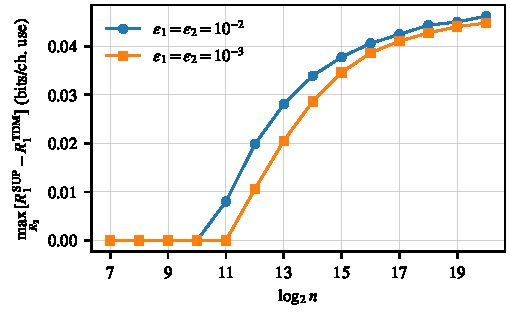
\includegraphics[width=\columnwidth]{figures/crossover.pdf}
\caption{Largest advantage in $R_1$ of $\Rs^{\mathrm{SUP}}$ over $\Rs^{\mathrm{TDM}}$ at equal $R_2$, for $\mathrm{BSBC}(0.01,0.10)$. A value of 0 means that the SUP region lies inside the TDM region.}
\label{fig:crossover}
\end{figure}

Fig.~\ref{fig:crossover} quantifies how long the blocklength must be for SUP to pay off. For each $n$, it shows the largest amount by which $\Rs^{\mathrm{SUP}}$ exceeds $\Rs^{\mathrm{TDM}}$ in $R_1$ at equal $R_2$. For $n\leq2^{10}$, the SUP region lies inside the TDM region for both reliability targets. Among the evaluated blocklengths (powers of two), SUP first extends beyond TDM at $n=2^{11}$ for $\varepsilon_1=\varepsilon_2=10^{-2}$ and at $n=2^{12}$ for $10^{-3}$. Its advantage then grows slowly, to about $0.045$~bits per channel use at $n=2^{20}$. Thus, on the BSBC, superposition coding needs blocklengths of thousands of bits before it outperforms TDM. At such blocklengths polarization is much more complete, and the main difficulty in constructing a polar superposition code becomes the estimation of the Bhattacharyya parameters~\cite{talvardy2013}, as in~\cite{CHOI2017111}. \reviewnote{Because the two regions share their endpoints, the plotted metric is clipped at~0 and hides how far SUP is behind at short $n$. The signed gap over interior rate pairs (per-stage approximation) is about $-0.10$ at $n=2^7$ and $-0.008$ at $2^{10}$ for $\varepsilon=10^{-2}$, which is more informative. The crossover is also robust to the third-order term: adding $\frac{1}{2}\log n/n$ to every constituent code keeps it at $2^{11}$ ($10^{-2}$) and $2^{12}$ ($10^{-3}$), in a per-stage approximation. Saying so would preempt an obvious reviewer question.} \reviewnote{Only one channel pair is evaluated, and its asymptotic SUP advantage over time sharing is just $0.048$ bits/use (maximized over $R_2$); at $n=2^{20}$, Fig.~\ref{fig:crossover} already reaches $96\%$ of it. Add the asymptote as a dashed line, and add a second BSBC with a larger asymptotic gain to show that the conclusion is not specific to this channel.}

\section{Conclusion}
\label{sec:conclusion}
We identified the challenges that a polar superposition code for the BSBC faces at finite blocklength, beyond those of P2P polar codes. We proposed a construction that combines a normal approximation for random SUP with the 5G NR reliability sequence. The construction performs adequately at $n=128$, but, consistent with the normal approximation, it does not outperform TDM with P2P polar codes; the normal approximation predicts that SUP needs blocklengths of thousands of bits to do so on this channel. Several directions remain open. Other codes can replace the polar cloud center; in preliminary experiments, a Reed--Muller cloud center slightly improved performance. \reviewnote{This claim has no supporting data in the paper; add a data point or remove it.} With $U_2^n$ fixed to zero, the satellite encoder becomes a generator of low-average-weight codes, which may be useful for secrecy, covertness, and uncoordinated multi-user access. Finally, the underperformance of SUP is likely due to the all-or-nothing interference of a binary input alphabet, in contrast with Gaussian downlink models~\cite{sun2018shortpacket}. This motivates extending the analysis to larger alphabets.

\bibliographystyle{IEEEtran}
\bibliography{refs}

\end{document}
